\documentclass{beamer-control}
\usepackage{beamer-control-singlefile}
\INCLUDEONLY{Basic Definitions}
\begin{document}
\CONCEPT{Basic Definitions}

\begin{SUMMARY}
\begin{itemize}
\item Linearity
\item Time invariance
\end{itemize}
\vfill References:
\begin{itemize}
\item \astrom{§6.1}
\end{itemize}
\end{SUMMARY}



\SUBCONCEPT{Linearity}

\begin{frame}
\frametitle{Static gain models}
\begin{itemize}
\item Vary input $r=10\%\dots100\%$ (say)
\item Record steady state output vs control input
\item For linear models, slope will be constant
\item For nonlinear models, non-constant slope
\item E.g., rubber or magnetic spring
\end{itemize}
\end{frame}


\begin{frame}[fragile]

\newcommand{\myfig}[6]{%
\begin{scope}[xshift=#6,
             spring/.style = {decorate,
                              decoration = {aspect         = 0.5,
                                            segment length = #1,
                                            amplitude      = 2mm,
                                            coil}}]

\path (0,0)                            coordinate (g)
      (0,-0.5cm)                       coordinate (topspring)
      (0,#2)                           coordinate (bottomspring)
      (bottomspring) ++(0,-.5cm)       coordinate (pt2)
                      +(0cm,-#3)       coordinate (pt3)
                      +(1.25cm,-#3)    coordinate (#5 pt3);

 \node [platform,
        anchor = south] at (g)  {};
 \draw [very thick]    (-1,0)         -- (1,0);
 \draw                (topspring)     -- (g)
                      (bottomspring)  -- (pt2.north);
 \draw [spring]       (bottomspring)  -- (topspring);
 \draw [] (pt3) circle (#3)
                          node[inner sep = 0,
                               scale     = #4,
                               text      = black]{$m_{#5}$};
% \node[right=1.5*#3] at (pt3) {#5} ;
 \end{scope}
}

\begin{tikzpicture}[thick,
                    every node/.style = {draw      = none,
                                         inner sep = 0pt,
                                         outer sep = 0pt},
                    platform/.style   = {fill,
                                         pattern = north east lines,
                                         minimum width  = 2cm,
                                         minimum height  =0.3cm}]
 \myfig{1mm}{-2cm}{0.20cm}{0.5}{A}{-2cm}
 \myfig{3mm}{-3cm}{0.28cm}{0.8}{B}{ 0cm}
 \myfig{3mm}{-4cm}{0.39cm}{1.1}{C}{ 2cm}

\draw[dashed]  (A pt3)  +(-0.4,0)     --               +(0.4,0)
                        +(-0.4+2,0) -- coordinate (b1) +(0.4+2,0)
               (B pt3)  +(-0.4-2,0) -- coordinate (a2) +(0.4-2,0)
               (C pt3)  +(-0.4-2,0) -- coordinate (b2) +(0.4-2,0) ;

\draw[latex-latex] (A pt3) -- node[right=0.1cm]{} (a2);
\draw[latex-latex] (b1)    -- node[right=0.1cm]{} (b2);

\end{tikzpicture}

\end{frame}


\begin{frame}
\frametitle{Linear vs Affine}

\begin{align}
m\ddot x &= -c\dot x - k (x-l_0) - mg + f
\end{align}
\begin{itemize}
\item What is the spring force for $x = l_0$ ?
\item What is the spring force at equilibrium $x_e$ ?
\item Note that 
\end{itemize}
\begin{align}
\Deriv{(x-l_0)}{t} =
\Deriv{(x-x_e)}{t} =
\Deriv{(x)}{t}
\end{align}
So:
\begin{align}
m\ddot {\tilde{x}} &= -c\dot{\tilde x} - k \tilde{x} + f
\end{align}

\end{frame}

\begin{frame}
\frametitle{Affine state space}
Translating systems to their equilibrium point is often \emph{required} due to the form of the state space equations:
\begin{align}
\Deriv{x}{t} = \Matr{\dot x\\\ddot x} = Ax + Bu = \Matr{0 & 1\\ -\frac km & -\frac cm } \Matr{x \\ \dot x} + Bu
\end{align}
Note that there is no constant term!\footnote{Let's just say we \emph{could} include it through  $Bu$  but it's not a good idea.}
\end{frame}

\begin{frame}
\frametitle{Linearity of solutions}
\begin{itemize}
\item<uncover@1-> Principle of superposition:
\begin{itemize}
\item Solution from scaled input $y(\alpha x_0)=\alpha y(x_0)$
\item Solution from multiple inputs $y(x_1+x_2)=y(x_1)+y(x_2)$
\item Etc.\ for $u$
\end{itemize}
\item<uncover@2-> Therefore we often consider:
\begin{itemize}
\item Solution to the homogeneous (or unforced) system \[\Deriv{x_h}{t}=Ax_h\]
\item Solution to the particular (or forced) system \[\Deriv{x_p}{t}=Ax_p+Bu\]
\item And their combinations --- see textbook Example 6.1
\end{itemize}
\end{itemize}
\end{frame}


\SUBCONCEPT{Time invariance}

\begin{frame}{Timey wimey}
Time invariance is a subtle concept:
\begin{itemize}
\item Of course solutions to $\Deriv{x}{t} = Ax$ are time-dependent
\item What we mean is $y_2(t+a) = y_1 (t)$ if $u_2(t+a) = u_1 (t)$
\end{itemize}
\end{frame}

\begin{frame}
\frametitle{Superposition across time}

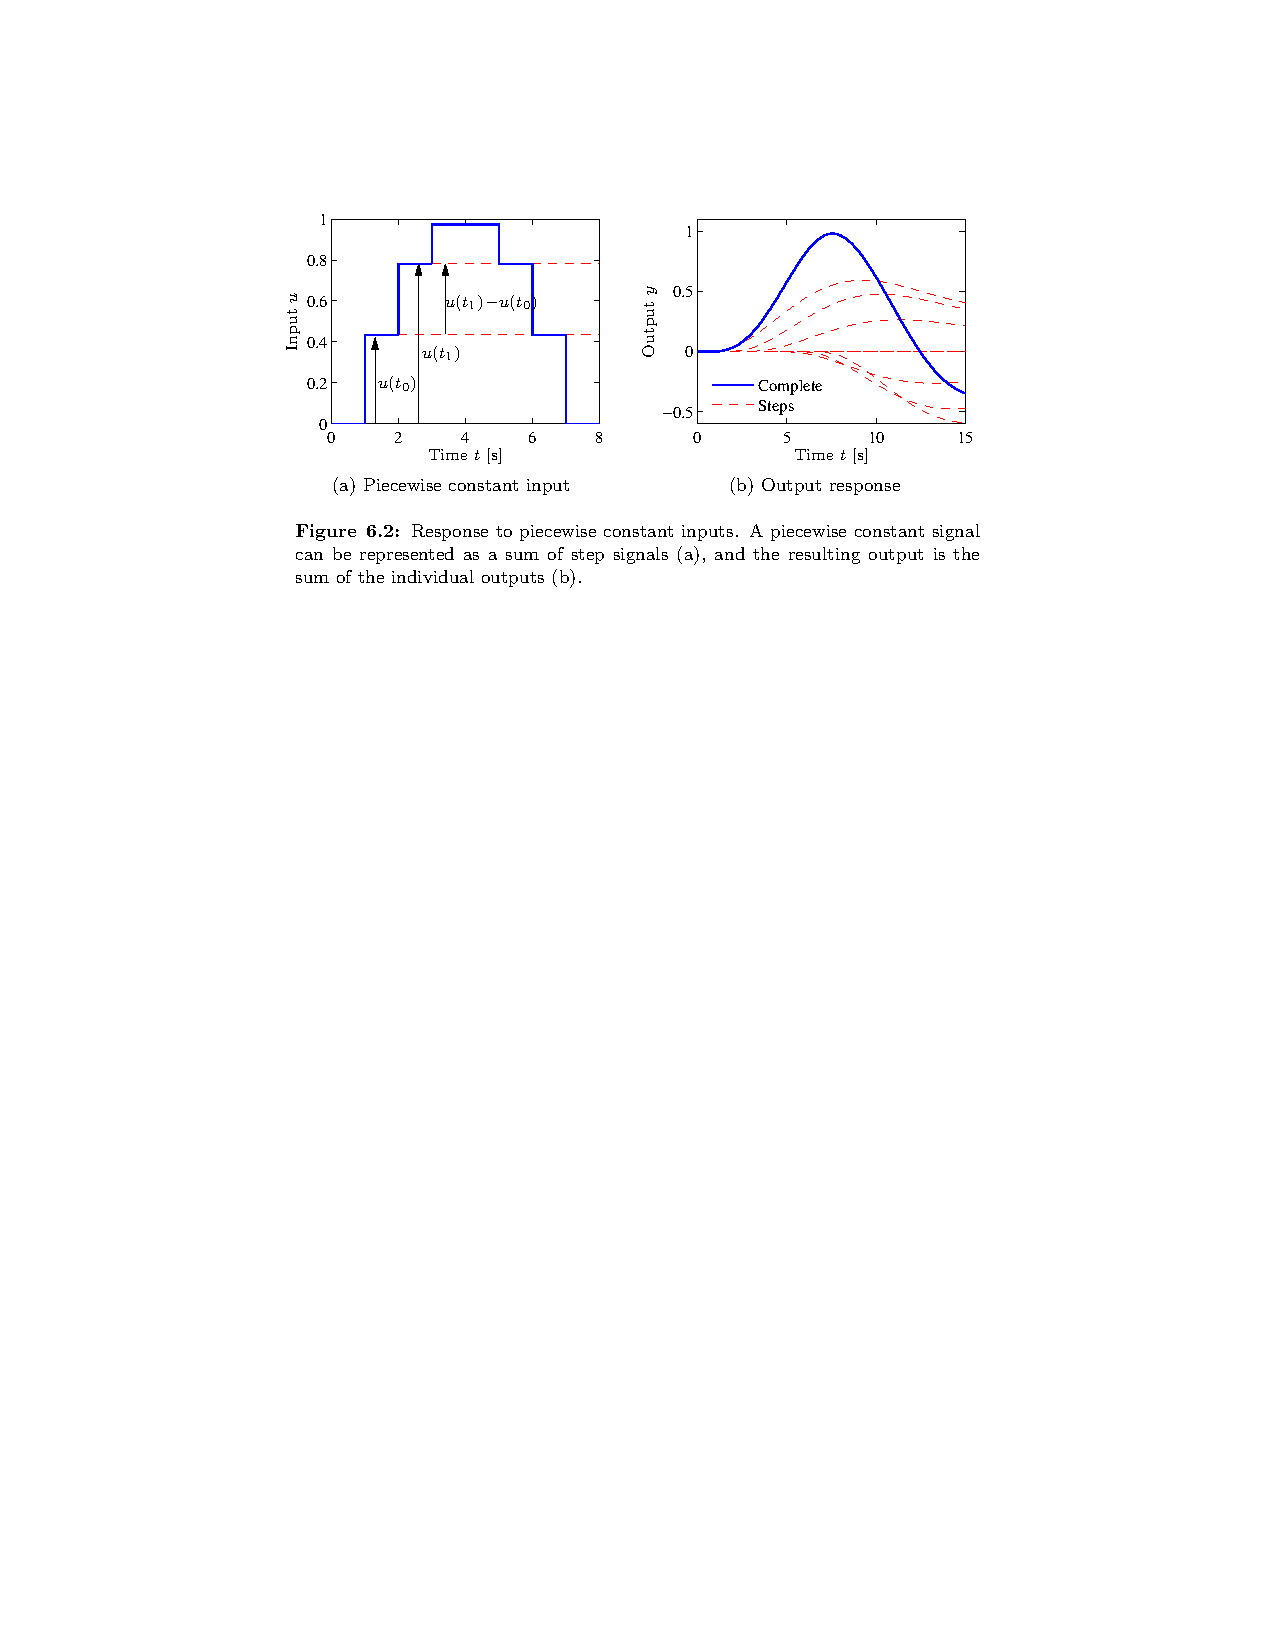
\includegraphics[width=\linewidth]{figure6.2}


\end{frame}

\begin{frame}
\frametitle{Introducing dirac $\delta(t)$}

Generalising the summation of discrete steps to an arbitrary input signal waveform:
\begin{align}\label{eq:imp}
u(t) = \int^t_0 \ImpulseInput(t-\tau)u(\tau)\dee\tau
\end{align}
where impulse input $\ImpulseInput(t)=S'(t)$ and $S(t)$ is a step input:
\begin{align}
S(t) &=
\begin{cases}
0 & t<0 \\
1 & t\ge 0
\end{cases}
&
\delta(t) &= 
\lim_{\varepsilon\to0}
\begin{cases}
0 & t<0 \\
\tfrac{1}{\varepsilon} & 0<t\le\epsilon \\
0 & t>\epsilon
\end{cases}
\end{align}

\end{frame}

\begin{frame}
\frametitle{Output of continuous signal}
We have:
\begin{align}\label{eq:imp}
u(t) = \int^t_0 \ImpulseInput(t-\tau)u(\tau)\dee\tau
\end{align}
This produces output response:
\begin{align}\label{eq:impresp}
y(t) = \int^t_0 \ImpulseResponse(t-\tau)u(\tau)\dee\tau
\end{align}
where impulse response $\ImpulseResponse(t)=\StepResponse'(t)$ and $\StepResponse(t)$ is step response.

\alert{\em The form of \eqref{impresp} is important for the following concepts.}

\end{frame}

\begin{frame}
\frametitle{LTI systems}
\begin{itemize}
\item When is a system not time invariant? Consider, e.g.:
\begin{itemize}
\item a rubber with stiffness that changes with temperature
\item non-Newtonian material with velocity-dependent damping
\item a rocket with fuel mass that burns away over time
\end{itemize}
\item All of classical control theory assumes we have linear, time-invariant (LTI) systems
\item These are generally \emph{good approximations} for most engineering systems
\item Errors due to these assumptions are often handled gracefully by the control system
\item Adaptive and/or nonlinear control is needed for more complex systems
\end{itemize}
\end{frame}

\SUMMARYFRAME
\FINALE

\end{document}
